
%(BEGIN_QUESTION)
% Copyright 2010, Tony R. Kuphaldt, released under the Creative Commons Attribution License (v 1.0)
% This means you may do almost anything with this work of mine, so long as you give me proper credit

The only active devices on the following FF H1 segment are the flow transmitter, the control valve, and the H1 interface card on the DCS I/O rack:

$$\includegraphics[width=15.5cm]{i04570x01.eps}$$

Supposing the H1 card on the DCS acts as the Link Active Scheduler (LAS) and that the PID control function resides in the control valve positioner, describe the sequence of events necessary to make the control loop work (i.e. reading the process variable signal, computing the controller output, moving the valve stem, updating setpoint from human operator).

\vskip 20pt \vbox{\hrule \hbox{\strut \vrule{} {\bf Suggestions for Socratic discussion} \vrule} \hrule}

\begin{itemize}
\item{} Suppose the LAS stops working.  How will this impact the operation of the Fieldbus segment?
\item{} Suppose the PID control function resides within the transmitter rather than in the valve positioner.  How would this affect the sequence of events on this H1 network segment?
\item{} Suppose this flow control loop is the ``slave'' (or ``secondary'') loop in a cascade control strategy, where some other controller on the FF segment is the ``master'' (``primary''), the output of this master PID function generating remote setpoint values for the flow controller.  How would the sequence of events change from what they are when the flow controller's setpoint comes from a human operator?
\end{itemize}

\underbar{file i04570}
%(END_QUESTION)





%(BEGIN_ANSWER)

\begin{itemize}
\item{$(1)$} LAS (DCS H1 card) issues a CD token to the flow transmitter
\item{$(2)$} Flow transmitter publishes the process variable (flow) value
\item{$(3)$} Control valve positioner receives (``subscribes to'') to the PV data
\item{$(4)$} PID algorithm compares PV with the last SP and calculates Output value
\item{$(5)$} Valve moves to match new Output value
\item{$(6)$} During unscheduled time, the LAS issues a Pass Token (PT) message to each device in turn
\item{$(7)$} At the valve positioner's turn, the PID algorithm requests new operator SP value from the DCS 
\item{$(8)$} At the DCS's turn, it transmits (``serves'') the new SP value to the PID algorithm
\end{itemize}

%(END_ANSWER)





%(BEGIN_NOTES)

If this flow controller were the slave in a cascade scheme, the setpoint would be broadcast using the Publisher/Subscriber VCR and as such it would happen on scheduled time:

\begin{itemize}
\item{$(1)$} LAS (DCS H1 card) issues a CD token to the flow transmitter
\item{$(2)$} Flow transmitter publishes the process variable (flow) value
\item{$(3)$} Control valve positioner receives (``subscribes to'') to the PV data
\item{$(4)$} LAS (DCS H1 card) issues a CD token to the master PID function block
\item{$(5)$} Master controller PID algorithm publishes its output as a remote SP value
\item{$(6)$} Control valve positioner receives (``subscribes to'') to the SP data
\item{$(7)$} PID algorithm compares PV with the SP and calculates Output value
\item{$(8)$} Valve moves to match new Output value
\item{$(9)$} During unscheduled time, the LAS issues a Pass Token (PT) message to each device in turn
\end{itemize}

%INDEX% Fieldbus, FOUNDATION (H1): Link Active Scheduler (LAS)
%INDEX% Fieldbus, FOUNDATION (H1): scheduled vs. unscheduled communication

%(END_NOTES)


